\documentclass[11pt, a4paper]{article}
%\documentclass[useAMS,referee]{biom}
\usepackage{graphicx}
\usepackage{amsmath, bm}
\usepackage{natbib}
\usepackage[utf8]{inputenc}    
\usepackage{natbib}
\usepackage[usenames,dvipsnames]{xcolor}
\usepackage[left=2cm,right=2cm,top=2cm,bottom=2cm]{geometry}
\usepackage{hyperref}
\usepackage[outdir=./]{epstopdf}
\usepackage{lscape}
\usepackage{float}  % PUT FIGURE HERE
\usepackage{array}  % fix column width 
\usepackage{caption}
\captionsetup[figure]{labelfont=bf}
\captionsetup[table]{labelfont=bf}
\usepackage{multirow}
\usepackage{booktabs} % Create TABS
\usepackage{array,longtable}
\title{Competitive gene set enrichment analysis for correlated expression data}
\date{} % Today's date or a custom date


\hypersetup{
	colorlinks,
	citecolor=blue,
	filecolor=blue,
	linkcolor=blue,
	urlcolor=blue
}



\begin{document}

	%  pub the summary here
	
	\begin{abstract}
		The world will little note, nor long remember, what we say here, but
		can never forget what they did here. It is for us, the living, rather
		to be dedicated here to the unfinished work which they have, thus far,
		so nobly carried out. It is rather for us to be here dedicated to the
		great task remaining before us--that from these honored dead we take
		increased devotion to that cause for which they here gave the last
		full measures of devotion--that we here highly resolve that these dead
		shall not have died in vain; that this nation shall have a new birth
		of freedom; and that this government of the people, by the people, for
		the people, shall not perish from the earth. The world will little
		note.
	\end{abstract}
	
	%
	%  Please place your key words in alphabetical order, separated
	%  by semicolons, with the first letter of the first word capitalized,
	%  and a period at the end of the list.
	%
	
%	\begin{keywords}
%		Colostrum; Milk; Milk oligosaccharide; Non-human mammal.
%	\end{keywords}
	
	\maketitle


	
	\section*{Abstract}
	To be filled
	
	\section{Introduction}\label{section:introduction}
	
	\textbf{What is enrichment analysis? Why would people care about that?}\\
	 \textit{Gene set test} is a method of studying the association between a set of genes, which are significantly correlated with treatment or experimental design variables, and a \textit{prior} set of genes, which are biologically related. A typical gene expression analysis involves the detection of a set of differentially expressed genes. Differential expression (DE) analysis  evaluates each individual gene separately, and therefore it fails to provide insight into the association of treatment variable with the gene set under study. Gene set test helps researchers better understand the underlying biological processes.
	 
	 	\textbf{What are the differences between self-contained and competitive test? And how does they work?}\\
	 Depending on the definition of the null hypothesis, there are two types of gene set test: the \textit{self-contained} test and the \textit{competitive} test \citep{goeman2007analyzing}. A self-contained test examines a set of genes by a fixed standard without reference to other genes in the genome (see \cite{goeman2004global,goeman2005testing, tsai2009multivariate, wu2010roast, huang2013gene} for example). A competitive test compares DE
	 genes in the test set to those not in the test set \citep{tian2005discovering, wu2012camera, yaari2013quantitative}. Many methods, regardless of the type of test, perform a three-stage analysis \citep{khatri2012ten}: on the first stage, a \textit{gene-level statistic} that measures the association between the expression profiles and the experimental design variables is calculated for each gene; such gene-level statistics include, among others, the \textit{signal-to-noise ratio} \citep{subramanian2005gene}, the ordinary \textit{$t$-statistic} \citep{tian2005discovering} or a moderated $t$-statistic \citep{Smyth2004moderated}, the \textit{log fold change} \citep{kim2005page} and the \textit{$Z$-score} \citep{efron2007correlation}. On the second stage, a \textit{set-level statistic} is summarized by using gene-level statistics and prior information about the test set (i.e., whether the gene belongs to the test set) as input. Examples of the set-level statistics are the \textit{enrichment score} \citep{subramanian2005gene}, the \textit{maxmean statistic} \citep{efron2007testing}, and statistic derived from joint distribution of gene-level statistics \citep{yaari2013quantitative}, to name a few. On the last stage, a $p$-value is assigned to the test set by comparing the set-level statistic to its reference distribution. The competitive gene set test is much more popular among genomic literatures \citep{goeman2007analyzing, gatti2010heading}.  
	 
	 %Competitive gene set test \citep{goeman2007analyzing} is a gene expression analysis that compares differential expression (DE) for genes in the test set to that for genes not in the test set. Most competitive gene set tests, as described by \cite{barry2008statistical}, are typically two-stage procedures:  on the second stage, a $p$-value is reported from the The test set may represent biological pathways or network, or some other grouping based on biological knowledge. Incorporating such prior information of the grouping makes it easier for biologists to interpret the results of DE analysis.
	
	\textbf{Independent gene set test} \\
	 Many competitive gene set test approaches rely on independence of gene-level statistics. Those tests are parametric or rank-based procedures that assume the gene-level statistics to be independent and identically distributed, or gene permutation procedures that generate the same approximate null for the set-level statistics. For example, PAGE  \citep{kim2005page} conducts one-sample $z$-test by comparing the mean of gene-level statistics (i.e., log fold changes) in the test set to a normal distribution under the null, assuming the  gene-level statistics to be independent. The $2\times 2$ contingency-table-based tests examine the significance of the test set by dichotomizing the outcomes of DE analysis and cross-classifying the genes according to whether they are indicated as DE and whether they are in the test set (see \cite{huang2009bioinformatics} for a review and references therein). sigPathway \citep{tian2005discovering} and "geneSetTest" in the limma package \citep{Smyth2004moderated} evaluate the set-level $p$-values by permuting gene labels. However, tests assuming independence of genes may result in inflated false discovery rate \citep{efron2007testing,goeman2007analyzing, gatti2010heading,wu2012camera,yaari2013quantitative},
	 as genes in a gene set are often correlated and function together.

	  \textbf{Tests that account for between-gene correlation}\\
	  A handful of methods have been proposed to account for between-gene correlation in competitive gene set test. One attempt is to evaluate the set-level statistic by permuting the biological samples (see, for example, \cite{subramanian2005gene, efron2007testing}). Permuting samples does not require an explicit understanding of the underlying correlation structure among genes and thus protects the test against such correlation. Since permuting sample labels is computationally inefficient, \cite{zhou2013empirical} proposed an analytic approximation to permutations for set-level score statistics, which preserves the essence of permutation gene set analysis with greatly reduced computational burden. (???seems not to be relevant to what we are talking about, should I move this to the discussion, or just delete it)  However, an unavoidable problem arising from sample permutation approach is that it implicitly alters the null hypothesis being tested and it is difficult to characterize the null and the alternative hypotheses \citep{goeman2007analyzing, khatri2012ten, 
	  	wu2012camera}. We will further discuss this point in later sections of this paper. Another attempt is to conduct set-level test that works with the between-gene correlation structures. \cite{wu2012camera} proposed Correlation Adjusted MEan RAnk (CAMERA) gene set test that first estimates a \textit{variance inflation factor} (VIF) associated with correlation between gene expression profiles, and then incorporates it into two versions (i.e., the parametric and the rank-based) of CAMERA tests. \cite{yaari2013quantitative} also used the idea of incorporating VIF to adjust for correlation in their distribution-based gene set analysis. Valid estimation of VIF relies on the assumption that correlation between any two local statistics are almost the same as correlation between their corresponding expression profiles. This assumption has been demonstrated (??? a better word???) by \cite{barry2008statistical} for several gene-level statistics (e.g., $t$-statistic, Wald-type statistic for regressing expression on censored time-to-event data through a Cox proportional hazards model). However, as shown by (the paper to be finished), this assumption holds only for the case where all of the gene-level tests are under the null (i.e., no gene is DE), and the correlation among gene-level statistics (e.g., $t$-statistics) can be badly estimated by sample correlation when a fraction of genes are DE. 
		% The CAMERA procedure thus may be too conservative for controling type I error in the presence of DE genes, as will be demonstrated in our simulation study. 

	   
	  % (This is a self-contained gene set test) \cite{huang2013gene} uses a multivariate linear regression model in which the between-gene correlation are explicitly modeled by a working covariance matrix. 
	
	\textbf{What do we propose?} \\
	In this paper, we propose a new competitive gene set test procedure that incorporates the correlation among gene-level statistics into the set-level test statistic. This procedure aims to correct for the discrepancy between correlation among expression profiles and that among gene-level statistics in the formulation of set-level statistic. The discrepancy is caused by the presence of DE genes for several typically used gene-level statistics (REF the paper to be finished). As a remedy, our strategy is to model the covariance matrix of gene-level statistics by two variance components, one attributable to the correlation among expression profiles and the other attributable to the DE effect associated with the treatment. OurMethod follows the three-stage paradigm and works for a two group comparison experiment under all correlation structures. Our simulations show that OurMethod controls type I error correctly and maintains good power for different correlation structures we examined. 
		
	\textbf{What is the plan of this paper?} \\
	The rest of the paper is organized as follows: in Section \ref{section:methods} we describe OurMethod.....
	
	
	
	\section{Methods}\label{section:methods}
	\textbf{Overview of this section} \\
	In the first part of this section, we will formulate our model: first, we introduce a DE effect for each gene, based on which we derive the correlation between our gene-level statistics; then we define the null and alternative hypotheses for competitive gene set test under this framework; next we propose our set-level test statistic and conduct hypothesis testing. In the second part, we will briefly summarize four different approaches that we will compare against in the result section.  
	
	\subsection{OurMethod}
	\subsubsection*{The DE effects}\label{subsection:DEeffect}

	In a treatment-control gene expression experiment, we denote by $Y_{ijk}$ a random variable for the expression level of gene $i$ from sample $j$ in treatment group $k$, with $i$ taking the values $1, \ldots, m$ (the number of genes), $j$ taking the values $1, \ldots, n_k$ (the total number of biological samples), and $k$ being either 1 for control or 2 for treatment. Correspondingly, $Y^{\ast}_{ijk}$ represents the standardized expression levels (described in REF???) for gene $i$ of sample $j$, with $Y^{\ast}_{ijk}\sim N(0, 1)$ (??? Normal assumption necessary here???)  if sample $j$ comes from the control group, and $Y^{\ast}_{ijk}\sim N(\Delta_i, 1)$ if it comes from the treatment group. Here, $\Delta_i$ is a \textit{DE effect}: compared to the control group,  gene $i$ is not DE if $\Delta_i=0$, up-regulated if $\Delta_i >0 $ and down-regulated if $\Delta_i<0$.
	% By "internal" we mean that every gene has a tendency to be DE with a random DE size $\Delta$, for example, for those stably-expressed genes $P(\Delta = 0) = 1$. 
	In a gene expression experiment, the DE effect $\Delta_i$ consists of two parts: I) the treatment which determines whether a gene is DE or not; and II) the DE effect size or strength when the gene is DE. 
	%We assume that the DE effects are mutually independent for all genes, and that whether gene $i$ is DE or not is determined by a DE "trigger" --- the treatment applied to gene $i$ in the experiment. 
	For I), we let $\bm Z = (Z_1, \ldots, Z_m)$ be a vector of DE indicators, where $Z_i=1$ if gene $i$ is DE and $Z_i = 0$ otherwise, and (DO WE NEED TO ASSUME $Z_i$s TO BE INDEPENDENT OF EACH OTHER?)
	\begin{equation}\label{eq:DEindicator}
		Z_i \sim \text{Binom}(1, p_i)
	\end{equation}
	For II), we denote $\delta_i$ as the \textit{DE effect size} for all genes $i$ and $\delta_i$ follows some distribution $ f_{\delta}$ with mean and variance
	\begin{equation}\label{eq:DEdistribution}
		E(\delta_i) = \mu_{\delta}, ~~\text{Var}(\delta_i) = \sigma^2_{\delta}
	\end{equation}
	We further assume that the DE indicator $Z_i$ is independent of the DE effect size $\delta_i$ for gene $i=1, \ldots, m$.  Therefore, the DE effect can be expressed as
	\begin{equation}\label{eq:DEeffect}
		\Delta_i = Z_i\delta_i,
	\end{equation}
	It can be shown that (details in Appendix \ref{section:appendix}), 
	\begin{equation}\label{eq:deltaMeanVar}
		E(\Delta_i) = p_i\mu_{\delta}, ~~  \text{Var}(\Delta_i)= p_i\sigma_{\delta}^2 + p_i(1-p_i)\mu_{\delta}^2, ~~i = 1, \ldots, m.
	\end{equation}
	
	
	We assume that conditioning on the DE effects, expression levels for different samples are independent, but expression levels for different genes of the same sample may be correlated. Denote by $\bm C_{m \times m}$ the gene correlation matrix, with entry $\rho_{i_1, i_2}$ being the correlation between gene $i_1$ and gene $i_2$. Note that the between-gene correlation $\rho_{i_1, i_2}$ is a constant, regardless of whether the sample is from the treatment or from the control group. In this paper, we estimate the between-gene correlation matrix $\bm C$ by the residual sample correlation after the treatment differences have been nullified (as done by \cite{efron2007correlation} and \cite{wu2012camera}).
	
	\subsubsection*{Gene-level statistics and their correlation}\label{subsubsection:genelevelcorrelation}
	
	We denote by $I_t$ and $I_b$ the test set and the \textit{background set} (i.e., the genes not in the test set). Let $\bm x = (x_1, \ldots, x_m)$ be a indicator vector, with $x_i=1$ if gene $i$ belongs to the test set and $x_i=0$ otherwise. Therefore $I_t = \{i: x_i =1\}$ and $I_b = \{i: x_i =0\}$. We assume that the DE probability is $p_t$ for genes in the test set and $p_b$ for genes in the background set. For gene $i$, the gene-level statistic is the difference in mean expression levels between the treatment and the control groups,
	\begin{equation}\label{eq:genelevelstat}
		U_i=\bar{Y}_{i.2}-\bar{Y}_{i.1}
	\end{equation} 
	where $\bar{Y}_{i.k}= \sum_{j=1}^{n_k}Y_{ijk}/n_k$. It follows from equation (\ref{eq:deltaMeanVar}) that $\bm U = (U_1, \ldots, U_m)$ has mean
	\begin{equation}\label{eq:expectation}
		E(U_i) = \left \{
		\begin{aligned}
			&p_t\mu_{\delta}, && \text{if}\ i \in I_t \\
			&p_b\mu_{\delta}, && \text{if}\ i \in I_b
		\end{aligned} \right.
	\end{equation} 
	and covariance matrix (see Appendix \ref{section:appendix} for detail) 
	\begin{equation}\label{eq:variance}
		\text{Var}(\bm U) = \bm D  + \sigma_2^2\bm C
	\end{equation}
	where $\bm D = \text{diag}(d_1, \ldots, d_m)$ with $d_i = p_t\sigma_{\delta}^2 + p_t(1-p_t)\mu_{\delta}^2$ if $i\in I_t$ and $d_i =p_b\sigma_{\delta}^2 + p_b(1-p_b)\mu_{\delta}^2$ if $i\in I_b$,  $\sigma_2^2 =\frac{1}{n_1} + \frac{1}{n_2} $ and $\bm C$ is the between-gene correlation matrix. 
	
	\subsubsection*{The null hypothesis for competitive gene set test}\label{subsubsection:nullhypothesis}
	For a competitive gene set test, it is often unclear what the hypothesed null is, and thus what is being tested (\cite{barry2008statistical}  \citealp{wu2012camera}). Note that the DE probability affects both the mean vector in equation (\ref{eq:expectation}) and the covariance in equation (\ref{eq:variance}). Under this framework, the test set is not enriched only if the probability of DE in the test set is the same as that in the background set. Therefore, the hypothesis for enrichment testing can be statistically formulated as
	\begin{equation}\label{eq:null}
		H_0\text{: }  p_t = p_b \stackrel{\text{def}}{=}p_0  \text{ Versus } H_1 \text{: } p_t \neq p_b
	\end{equation}
	We can combine equations (\ref{eq:expectation}) and (\ref{eq:variance}) into the following linear model
	\begin{equation}\label{eq:linearModel}
		\bm U = \beta_0\bm 1_m + \beta_1\bm x + \bm \epsilon, \text{~~Cov}(\bm \epsilon) =  \bm D  + \sigma_2^2\bm C
	\end{equation} 
	with $ \beta_0 = p_b\mu_{\delta}, ~\beta_1 = (p_t-p_b)\mu_{\delta}$ and $\bm 1_m$ being a vector of ones. Now the hypothesis testing problem in (\ref{eq:null}) becomes 
	\begin{equation}\label{eq:linearHypothesis}
		H_0\text{: }  \beta_1 = 0   \text{ Versus } H_1 \text{: } \beta_1 \neq 0.
	\end{equation}
	Under the null of (\ref{eq:linearHypothesis}), we have $E(\bm U) = \beta_0\bm 1_m$ and $\text{Var}(\bm U) = \sigma^2_1\bm I_m + \sigma_2^2 \bm C$ where $\bm I_m$ is an identity matrix and $\sigma_1^2 = p_0\sigma^2_{\delta}+ p_0(1-p_0)\mu^2_{\delta}$.
	
	\subsection*{Set-level statistic}\label{subsection:setlevelstat}
	In practice, we need to estimate $\beta_0, \beta_1,\sigma_1^2$ and $\bm C$ in model (\ref{eq:linearModel}) for gene set test. Our strategy is to use \textit{quasi-likelihood}, which requires only the mean and the variance of $\bm U$.  The between-gene correlation matrix $\bm C$ is estimated by the residual sample correlation after the treatment differences have been nullified, and is treated as known in estimating $\beta_0$ and $\sigma_1^2$. 
	Denoting by $\hat{\bm C}$ the estimate of $\bm C$ and,
	\begin{equation}\label{eq:estimateparameter}
		\bm\Sigma = \sigma^2_1\bm I_m + \sigma_2^2 \hat{\bm C}
	\end{equation}
	The score equations for $\beta_0$ and $\sigma_1^2$ are
	\begin{equation}
		\begin{aligned}
			(\bm U - \beta_0\bm 1_m)^T \bm \Sigma^{-1}\bm 1_m & = 0\\
			(\bm U - \beta_0\bm 1_m)^T \bm \Sigma^{-1} \hat{\bm C} (\bm U - \beta_0\bm 1_m) &= \text{trace}(\bm \Sigma^{-1}\hat{\bm C})
		\end{aligned}
	\end{equation}
	\textbf{.... something to catch up.....}\\
	The enrichment test statistic for the test set is 
	\begin{equation}\label{eq:teststatistic}
		T = \frac{\left[\bm x^T(\bm U - \hat{\beta}_0 \bm 1_m )\right]^2}{\left[\bm x^T(\bm I - \bm H)\right]\bm \Sigma \left[\bm x^T(\bm I - \bm H)\right]^T}
	\end{equation} 
	Under the null, $T\sim \chi^2(1)$.
	
	
	\subsection{Other competitive gene set tests}
	We will compare OurMethod to five existing gene set tests: Gene set enrichment analysis (GSEA, \cite{subramanian2005gene}), two versions of the CAMERA procedure \citep{wu2012camera}, two versions of the geneSetTest procedure, and QuSAGE \citep{yaari2013quantitative}. All tests but geneSetTest account for correlation among genes. We will denote the two versions of CAMERA by CAMERA-modt and CAMERA-rank. The first version of geneSetTest, denoted by \textit{geneSetTest-modt}, is similar to sigPathway \citep{tian2005discovering} except it uses moderated $t$-statistics instead of the ordinary $t$-statistics as gene-level statistics. The second version of geneSetTest is also known as the mean rank gene set enrichment \citep{michaud2008integrative} and will be referred to herein as MRGSE. GSEA is modified from the original R-GSEA script (\url{http://software.broadinstitute.org/gsea/index.jsp}) to accommodate single gene set test. CAMERA and geneSetTest are implemented  in the limma package \citep{smyth2005limma} in the Bioconductor project \citep{gentleman2004bioconductor}, and QuSAGE in the Bioconductor package of the same name. Because GSEA and OurMethod do not support linear models, the implementations are restricted to two-group comparisons.
	
	The five tests differ in one or more respect. Except QuSAGE, all tests follow the three-stage paradigm, yet they are different on one or more stages. For GSEA, the gene-level statistics are the rankings of genes according to a ranking metric (we use signal-to-noise ratio, the default metric in R-GSEA), then based on the rankings an enrichment score for the test set is calculated, and the significance of the enrichment score is determined by randomly permuting the sample labels. Both CAMERA-modt and geneSetTest-modt use the moderated $t$-statistics \citep{Smyth2004moderated} as gene-level statistics, and determine whether the means of the gene-level statistics are significantly different for genes in the test set versus genes in the background set. The difference is how they evaluate the set-level statistics: CAMERA-modt uses a $t$-statistic that allows the gene-level statistics in the test set to be correlated by first estimating a variance inflation factor, and then incorporating it into the $t$-statistic to adjust for between-gene correlation (see materials and methods section of \cite{wu2012camera}); geneSetTest-modt evaluates the significance of the test set by comparing the observed set-level statistics to its null distribution generated by permuting gene labels. CAMERA-rank and geneSetTest-rank conduct a Wilcoxon-Mann-Whitney rank sum test, and they amount to, respectively,  CAMERA-modt and geneSetTest-modt in that they compare the rankings instead of the gene-level statistics themselves for genes in the test set to those for genes in the background set. QuSAGE generates from $t$-test a probability density function (PDF) for each gene, combines the individual PDFs using convolution, and quantifies gene-set activity with a complete PDF. The complete PDF can be used to compare a baseline value for self-contained gene set test, or to compare differences in expression between test set and background set in competitive gene set test.  
	

	
	\section{Examples and Numerical Results}\label{section:results}

	\subsection{Simulations}\label{subsection:simulation}
		In this section, we present results from type I error and power simulations under a range of between-gene correlation structures.
		
		The simulations run as follows: first, we simulate an entire gene set containing $m=500$ genes, from which we randomly sample $m_1 = 100$ genes to represent those in the test set, and the remaining $m_2=400$ genes belong to the background set; second, for gene $i=1, \ldots, m$, we simulate the DE effect $\Delta_i$ by first generating the DE size $\delta_i$ from $N(0.2, 1)$ and the DE indicator $Z_i$ from $\text{Binom}(1, p_i)$,  where $p_i= p_t$ if gene $i$ belongs to the test set and $p_i = p_b$  otherwise, and then setting $\Delta_i$ to be the product of $Z_i$ and $\delta_i$; third, we set the "true" mean expression values $\mu_1 = \bm 0_m$ and $\bm \mu_2 = \bm \Delta$, respectively,  for the control and treatment groups; fourth, we simulate $n_1$ samples from $\text{MVN}(\bm \mu_1, \bm \Sigma)$ for the control group and $n_2$ samples from $\text{MVN}(\bm \mu_2, \bm \Sigma)$, where the covariance $\bm \Sigma = (\sigma_{i_1, i_2})_{m\times m} $ may take one of the following forms: 
		\begin{enumerate}
			\item[(a0):] the genes are independent of each other (i.e., $\bm \Sigma = \bm I_m$).
			\item[(a):] only the genes in the test set are correlated, with exchangeable correlation structure, that is, $\text{Cor}(Y_{i_1}, Y_{i_2})=\sigma_{i_1, i_2}=\rho$ for $\forall i_1, i_2 \in I_t$ and  $\text{Cor}(Y_{i_3}, Y_{i_4})=\sigma_{i_3, i_4}=0$ if at least one of $i_3, i_4$ does not belong to $I_t$.
			\item[(c):] all genes are correlated, with exchangeable correlation structure, that is, $\text{Cor}(Y_{i_1}, Y_{i_2})=\sigma_{i_1, i_2}=\rho$ for $\forall i_1, i_2 \in I$.
			\item[(e):] genes are correlated within the test set and within the background set; but any two genes, one from the test set and the other from the background set, are independent. That is, the correlation structure is block diagonal, with $\text{Cor}(Y_{i_1}, Y_{i_2})= \sigma_{i_1, i_2}= \rho_1$ for $i_1, i_2 \in I_t$  , $\text{Cor}(Y_{i_3}, Y_{i_4}) = \sigma_{i_3, i_4}=\rho_2$ for $i_3, i_4\in I_b$, and  $\text{Cor}(Y_{i_5}, Y_{i_6})=\sigma_{i_5, i_6}= 0$ for $\forall ~i_5\in I_t, \forall~ i_6\in I_b$.
			\item[(f):] all genes are correlated, but the correlation between two genes depend on whether they belong to the test set or not. Specifically, $\text{Cor}(Y_{i_1}, Y_{i_2})=\sigma_{i_1, i_2}=\rho_1$  for $i_1, i_2 \in I_t$,    $\text{Cor}(Y_{i_3}, Y_{i_4})=\sigma_{i_3, i_4} =\rho_2$, for $ i_3, i_4\in I_b$, and  $\text{Cor}(Y_{i_5}, Y_{i_6})= \sigma_{i_5, i_6}= \rho_3$ for $\forall~ i_5\in I_t, \forall~ i_6\in I_b$.
		%	\item[(g):] genes are correlated in the same way as those from a real data.
		\end{enumerate}
		
		
		\subsubsection*{Type I error simulations}
		  
		   In the above simulation setup, the test set is not enriched if DE probabilities are the same for the genes in the test set and for those in the background set (i.e., $p_t = p_b = p_0$). However, it is shown in (the paper to be finished) that the test statistics correlation between two genes is not equal to their sample correlation when at least one gene is truly DE (under two sample $t$-test???). Therefore, if there are true DE genes in the entire gene set, approaches assuming the same correlation between gene-level statistics and between expression values may not perform well. To illustrate this point, we performed two groups of simulations for each of the correlation structures above: in group $A_1$, we simulated expression data with no DE genes, that is, $p_t = p_b = 0$; and in group $A_2$, we simulated data sets with the same DE probabilities for all genes --- specifically, DE probabilities are the same for genes in the test set and for those in the background set with $p_t= p_b = 0.2$. 
		 
		  For group $A_1$, Figure \ref{fig:typeIerror} shows the histograms of type I error rates for the six approaches (OurMethod, geneSetTest-modt, geneSetTest-rank, CAMERA-modt, CAMERA-rank and GSEA) under the six correlation structures. OurMethod and GSEA hold the size of type I error rates correctly for all 6 correlation structures, with simulated $p$-values uniformly distributed on $[0, 1]$. The two version of CAMERA control type I errors correctly for correlation structures (a0) and (a). However, both are too conservative for the case of (c) and (g), and anti-conservative for correlation structures (e) and (f). geneSetTest procedures may be too liberal depending on the underlying correlation structures. 
		  
		 For group $A_2$ simulation where DE probabilities are 0.2 across all genes, we summarize the results of the type I error rate simulation in Table \ref{table:typeIerror}. OurMethod continues to hold the size of type I error rates under all six correlation structures. However, GSEA is highly skewed towards small $p$-values and the two versions of CAMERA procedures are too conservative under all correlation structures, and the only exception is that CAMERA controls type I error rates correctly for (a0) where genes are simulated to be independent. The two versions of geneSetTest performs reasonably well.
		 
		 
		 \textbf{Explain why this happens}\\
		OurMethod shows consistent accuracy for type I error control across all simulations, but the accuracy of the other three methods may be affected by two factors: the between-gene correlation structures, and DE probability of each gene. OurMethod controls the size of type I error rates well because it takes into account the between-gene correlation and works directly with the sample correlation between genes, and therefore is robust against the two factors. (rewrite from here, because this is only my understanding.)  The GSEA evaluates the enrichment score of a test set by generating its null distribution from sample permutation, and therefore the between-gene correlation is preserved when there are no DE genes, but [ explain when DE exists]... 
		For CAMERA, the set-level statistics take into account only the between-gene correlation in the test set, and therefore does not work for cases where genes in the background set are also correlated in group $A_1$ simulations. More importantly, according to (the paper to be finished), the variance inflation factor of the gene-level statistics (moderated $t$-test in \cite{wu2012camera}) may be over-estimated when a fraction of genes are DE, and therefore the set-level test statistic is under-estimated, resulting in conservative $p$-values in group $A_2$ simulations. geneSetTest permutes the gene labels to examine the significance of the test set, and therefore it relies on independence between genes. The performances of both versions of geneSetTest are thus unpredictable in group $A_1$. In group $A_2$ where there are DE genes both in the test set and in the background set, the correlation between the gene-level statistics are smaller (in absolute value) than the correlation between the genes. Since the genes are simulated to be slightly correlated ($\rho_1=0.1, \rho_2 = 0.05, \rho_3 = -0.05$), the correlation between the gene-level statistics are almost negligible for geneSetTest procedure. 
			

		\begin{figure}[H]
			\caption{Type I error rates for gene set tests, $p$-value distribution for case (a0) - (f) from left to right, from top to bottom, NO gene is DE}\label{fig:typeIerror}
	 \begin{center}
		\includegraphics[width=8cm,height=4.5cm]{Figures/a0_SizePoint1_0PCT.eps}
		\includegraphics[width=8cm,height=4.5cm]{Figures/a0_SizePoint1_10PCT.eps}
		\includegraphics[width=8cm,height=4.5cm]{Figures/a_SizePoint1_0PCT.eps}
		\includegraphics[width=8cm,height=4.5cm]{Figures/a_SizePoint1_10PCT.eps}
		\includegraphics[width=8cm,height=4.5cm]{Figures/c_SizePoint1_0PCT.eps}
		\includegraphics[width=8cm,height=4.5cm]{Figures/c_SizePoint1_10PCT.eps}
		\includegraphics[width=8cm,height=4.5cm]{Figures/e_SizePoint1_0PCT.eps}
		\includegraphics[width=8cm,height=4.5cm]{Figures/e_SizePoint1_10PCT.eps}
		\includegraphics[width=8cm,height=4.5cm]{Figures/f_SizePoint1_0PCT.eps}
		\includegraphics[width=8cm,height=4.5cm]{Figures/f_SizePoint1_10PCT.eps}
			\end{center} 
		\end{figure} 
		

		
%\begin{table}[ht]
%	\centering
%	\caption{Type I error rate of gene set tests for correlated expression values }\label{table:typeIerror}
%	\begin{tabular}{lrrrrlrrrr}
%		\hline
%		\cline{1-10}
%		\multicolumn{1}{l}{Method} &\multicolumn{4}{c}{Norminal $p$-values}&  & \multicolumn{4}{c}{Norminal $p$-values} \\ \cline{2-10} 
%		 & 0.01 & 0.05 & 0.1 & 0.2 &    & 0.01 &0.05 & 0.1 & 0.2 \\ 
%		\hline
%		  & \multicolumn{4}{c}{(a0)} & & \multicolumn{4}{c}{(a)} \\
%		OurTest & 0.012 & 0.066 & 0.124 & 0.241 &  & 0.011 & 0.049 & 0.097 & 0.198 \\ 
%		geneSetTest-modt & 0.012 & 0.058 & 0.109 & 0.215 &  & 0.006 & 0.052 & 0.099 & 0.219 \\ 
%		geneSetTest-rank & 0.012 & 0.055 & 0.110 & 0.214 &  & 0.018 & 0.060 & 0.116 & 0.202 \\ 
%		CAMERA & 0.006 & 0.059 & 0.135 & 0.217 &  & $<0.001$ & $<0.001$ & $<0.001$ & 0.006 \\ 
%		CAMERA-Rank & 0.003 & 0.054 & 0.112 & 0.229 &  & 0.001 & 0.009 & 0.023 & 0.079 \\ 
%		GSEA & 0.989 & 0.995 & 0.997 & 0.997 &  & 0.228 & 0.608 & 0.794 & 0.927 \\ 
%			 & \multicolumn{4}{c}{(c)} &  & \multicolumn{4}{c}{(e)} \\
%		OurTest & 0.007 & 0.052 & 0.103 & 0.202 &  & 0.008 & 0.056 & 0.093 & 0.207 \\ 
%		geneSetTest-modt & 0.007 & 0.051 & 0.098 & 0.187 &  & 0.015 & 0.058 & 0.106 & 0.217 \\ 
%		geneSetTest-rank & 0.006 & 0.050 & 0.106 & 0.190 &  & 0.024 & 0.082 & 0.138 & 0.225 \\ 
%		CAMERA & $<0.001$ & $<0.001$ & $<0.001$ & $<0.001$ &  & $<0.001$ & $<0.001$ & 0.001 & 0.009 \\ 
%		CAMERA-Rank & $<0.001$ & $<0.001$ & $<0.001$ & $<0.001$ &  & $<0.001$ & 0.020 & 0.054 & 0.127 \\ 
%		GSEA & 0.942 & 0.984 & 0.992 & 0.995 &  & 0.108 & 0.469 & 0.731 & 0.899 \\ 
%			 & \multicolumn{4}{c}{(f)} & & \multicolumn{4}{c}{(g)} \\
%		OurTest & 0.012 & 0.050 & 0.098 & 0.226 &  & 0.007 & 0.059 & 0.116 & 0.211 \\ 
%		geneSetTest-modt & 0.010 & 0.071 & 0.115 & 0.213 &  & 0.010 & 0.061 & 0.104 & 0.218 \\ 
%		geneSetTest-rank & 0.007 & 0.061 & 0.112 & 0.221 &  & 0.014 & 0.072 & 0.142 & 0.247 \\ 
%		CAMERA & $<0.001$ & $<0.001$ & 0.004 & 0.019 &  & $<0.001$ & $<0.001$ & 0.001 & 0.006 \\ 
%		CAMERA-Rank & 0.006 & 0.041 & 0.096 & 0.210 &  & $<0.001$ & $<0.001$ & 0.002 & 0.009 \\ 
%		GSEA & 0.015 & 0.188 & 0.434 & 0.770 &  & 0.943 & 0.975 & 0.983 & 0.992 \\ 
%		\hline
%	\end{tabular}
%\end{table}


		\subsubsection*{Power simulation}\label{subsection:power}		 
		  Similar to the type I error simulation, we did two groups of simulations to get a glimpse into the power issues: in group $A_3$, we considered four different alternative scenarios by setting DE probability to be $0\%$ for genes in the background set and $5\%, 10\%, 15\%$ and $20\%$ for genes in the test set; in group $A_4$, we set DE probability to be $10\%$ for genes in the background set and $15\%, 20\%, 25\%$ and $30\%$ for genes in the test set. In both groups of simulation, we fixed the DE size $\delta$ for each alternative and the six different correlation structures. The power simulation were done by generating a large number of data sets under each alternative scenario and comparing the proportion of data sets for which each test would reject at a given level $\alpha$. 
		 
		 We compare the power of OurMethod to that of the other (How many methods) under different correlation structures. Since some of these tests are not well calibrated at the sample size considered (see Section \ref{subsection:typeIerror}), we report calibrated power. For calibrated power, the critical value $c(\alpha)$ is chosen so that when the null hypothesis is true, exactly $100\cdot\alpha\%$ of the resulting $p$-values are less than $c(\alpha)$; that is, $c(\alpha)$ is  the $\alpha$ quantile of null distribution of $p$-values, where the null distribution is generated from simulation. Calibrated power allows a more fair comparison among tests, as tests that are too conservative under the null hypothesis will have greater power due to the tendency to produce small $p$-values, yet this apparent power does not truly distinguish between the null and the alternative.  
		 
		  Table \ref{table:power1} and Table \ref{table:power2} summarize the calibrated power under correlation structure a0 (for power comparisons under the other five correlation structures, see online supplementary materials). In Table \ref{table:power1} we set the DE size $\delta$ to be 0.05 and simulated data in the way that genes in the background set are not DE (i.e., $p_b=0$). GSEA has the highest calibrated power, and the rank based MRSGE has the lowest calibrated power across all four alternative scenarios. CAMERA and OurMethod have virtually no difference in the calibrated power.  Furthermore, when the DE probability is $10\%$ or higher, both CAMERA and OurMethod have comparable calibrated power to that of GSEA. In Table \ref{table:power2}, we set the DE size $\delta$ to be 0.1 and simulated data with $10\%$ of the genes in the background set to be DE. CAMERA and OurMethod still have indistinguishable calibrated power and both are better than MRSGE. GSEA has virtually no power at all. These results indicate that....
		  
		  		
	% latex table generated in R 3.2.0 by xtable 1.8-0 package
	% Sat Feb 20 19:49:34 2016
	\begin{table}[ht]
		\centering
			\caption{power simulation results, NO DE}\label{table:power1}
		\begin{tabular}{rrrrr}
			\hline
		
		Method & \multicolumn{4}{c}{DE size = 0.1} \\
			\cline{2-5}
			& 5\% VS 0\% & 10\% VS 0\% & 15\% VS 0\% & 20\% VS 0\% \\ 
			\hline 
		OurTest & 0.654(0.005) & 0.956(0.002) & 0.998(0.000) & 1.000(0.000) \\ 
		MRSGE & 0.186(0.004) & 0.426(0.005) & 0.701(0.005) & 0.889(0.003) \\ 
		Camera & 0.647(0.005) & 0.953(0.002) & 0.998(0.000) & 1.000(0.000) \\ 
		GSEA & 0.827(0.004) & 0.991(0.001) & 1.000(0.000) & 1.000(0.000) \\ 
		QUSAGE & 0.723(0.004) & 0.974(0.002) & 0.999(0.000) & 1.000(0.000) \\ 
			\hline 
		\end{tabular}
	\end{table}
	
	
	% latex table generated in R 3.2.0 by xtable 1.8-0 package
	% Sat Feb 20 19:50:54 2016
	\begin{table}[ht]
		\centering
	    \caption{power simulation results, 10\% DE }\label{table:power2}
		\begin{tabular}{rrrrr}
			\hline
		Method & \multicolumn{4}{c}{DE size = 0.1} \\
			\cline{2-5}
			& 15\% VS 10\% & 20\% VS 10\% & 25\% VS 10\% & 30\% VS 10\% \\ 
			\hline
	OurTest & 0.229(0.004) & 0.604(0.005) & 0.871(0.003) & 0.976(0.002) \\ 
	MRSGE & 0.183(0.004) & 0.423(0.005) & 0.700(0.005) & 0.887(0.003) \\ 
	Camera & 0.227(0.004) & 0.596(0.005) & 0.864(0.003) & 0.973(0.002) \\ 
	GSEA & 0.000(0.000) & 0.000(0.000) & 0.000(0.000) & 0.000(0.000) \\ 
	QUSAGE & 0.244(0.004) & 0.630(0.005) & 0.889(0.003) & 0.981(0.001) \\ 
		\hline
		\end{tabular}
	\end{table}
	
	
	\begin{table}
		\centering
		 \caption{power simulation results, 10\% DE }\label{table:power}
		 	\begin{tabular}{rrrr c rrr}
		 		\hline\hline
		  & \multicolumn{3}{c}{DE size = 0.1} &  & \multicolumn{3}{c}{DE size = 0.1} \\
		 	Method & 5\% VS 0\% & 10\% VS 0\% & 15\% VS 0\%	 & & 15\% VS 10\% & 20\% VS 10\% & 25\% VS 10\% \\ 
		 	 \cline{2-4}   \cline{6-8}
		 	OurTest & 0.654(0.005) & 0.956(0.002) & 0.998(0.000) & & 0.229(0.004) & 0.604(0.005) & 0.871(0.003)\\ 
		 	MRSGE & 0.186(0.004) & 0.426(0.005) & 0.701(0.005)& & 0.183(0.004) & 0.423(0.005) & 0.700(0.005) \\ 
		 	Camera & 0.647(0.005) & 0.953(0.002) & 0.998(0.000)& & 0.227(0.004) & 0.596(0.005) & 0.864(0.003)  \\ 
		 	GSEA & 0.827(0.004) & 0.991(0.001) & 1.000(0.000) & & 0.000(0.000) & 0.000(0.000) & 0.000(0.000) \\ 
		 	QUSAGE & 0.723(0.004) & 0.974(0.002) & 0.999(0.000) & &  0.244(0.004) & 0.630(0.005) & 0.889(0.003) \\ 
		\hline
	\end{tabular}
\end{table}

	
	
		Figure \ref{fig:power} shows for OurMethod, the variations in power according to different correlation structures across four alternative scenarios. The left part is the power for group $A_3$ with a DE size of 0.05, and the right part is the power for group $A_4$ with a DE size of 0.05. For each correlation structure and each alternative, we simulated 1000 data sets and calibrated the power at a significance level of 0.05. 
		The powers for case (a0) and (c) are very similar, and are among the highest under each of the four alternatives. It's not surprising because they correspond to the simplest correlation structures: gene expression values in (a0) are simulated to be independent and in (c) are simulated to have the same correlation 0.1. As the correlation structure becomes more complicated, from (a) to (e) then to (f), the power decreases under every alternative scenario. The power under correlation structure (f) is the lowest for both $A_3$ and $A_4$ simulations. We also note that the power decreases when DE genes are present in the background set as compared to the case where there are no DE genes in the background set. (We might need the same DE size to illustrate this point.)
		
			\begin{figure}[H]
				\caption{power: left, DE size = 0.05, and no DE genes in the background set; right; DE size = 0.05, DE probability is 0.1 in the background set.}\label{fig:power}
				\begin{center}
					\includegraphics[width=8cm,height=5cm]{Figures/powerBack0pct.eps}
					\includegraphics[width=8cm,height=5cm]{Figures/powerBack10pct.eps}
				\end{center} 
			\end{figure} 
		
		\subsection{Real Data}
		We applied OurMethod to two example data sets, and compare the enriched gene sets to those obtained by GSEA and by CAMERA. In both examples, OurMethod are able to identify more enriched gene sets. Our results lend credence to previous studies in finding potential gene sets correlated with Huntington's disease and those correlated with chromosome Y and Y bands in lymphoblastoid cells.  
		
		\subsubsection*{Huntington's Disease Data}
		 We examined the Huntington's Disease (HD) RNA-Sequencing (RNA-Seq) data 	\citep{labadorf2015rna}  to identify which gene sets are enriched among DE genes in HD. The mRNA expression profiles in human prefrontal cortex were obtained from 20 Huntington's Disease samples and 49 neurologically normal controls.  Expression values were normalized and filtered as described in the methods section of \citep{labadorf2015rna}.
		 The data is available as a series GSE64810 in the GEO database (\url{http://www.ncbi.nlm.nih.gov/geo/}). The data set contains $28,087$ genes and the genes were named by their ensembl IDs. We performed enrichment analysis using the MsigDB \citep{subramanian2005gene} C2 Canonical Pathways gene sets (February 5, 2016, data last accessed). The C2 Canonical Pathway gene sets have a collection of 1330 gene sets, with an average set size of 50 (the set sizes range from 3 to 1028, and the median is 29). Since the genes in C2 Canonical Pathway gene sets are named by HGNC symbols, we converted the ensembl IDs in the expression data into HGNC symbols using \textit{BioMart} (\url{http://uswest.ensembl.org/biomart/martview/}). We retained $26,941$ genes that have corresponding HGNC symbols. For OurMethod, we standardized the data in the way as described in Section....
		 
		 
		 We used three test procedures (OurMethod, GSEA and CAMERA) to run enrichment analysis for the entire C2 Canonical Pathway gene sets, and compare the three tests in terms of resulting enriched gene sets. OurMethod found 176 out of 1330 gene sets to be enriched using the Benjamini-Hochberg (BH) procedure at a false discovery rate (FDR) of 0.05 (for multiple hypothesis testing, unless specified otherwise, all $p$-values in Real Data section are adjusted by BH procedure). GSEA found 9 enriched gene sets---8 of them are also among the 176 gene sets we identified (the one that is not significant according to OurMethod has a $p$-value of 0.008026062 and FDR 0.05739066). CAMERA found no enriched gene sets. In Figure \ref{fig:HDdatap} we present pairwise $p$-value plots for OurMethod, GSEA and CAMERA. When plotted against $p$-values of GSEA, for OurMethod, smaller $p$-values (e.g., less than 0.1) are more likely to cluster---as compared to larger $p$-values; that is, OurMethod produces significantly more small $p$-values than GSEA does while OurMethod and GSEA do not differ much in producing larger $p$-values.
		 The $p$-values of CAMERA are overwhelmingly larger than their counterparts of OurMethod, even if $p$-values of the two methods are highly correlated (Pearson's correlation is 0.96). This is consistent with our argument earlier (REF before) that CAMERA may be too conservative in practice. There is no systematic difference in $p$-values of GSEA and those of CAMERA. 
		 		 	\begin{figure}[H]
		 		 		\caption{raw p value plots for different methods}\label{fig:HDdatap}
		 		 		\begin{center}
		 		 			\includegraphics[width=5.5cm,height=5cm]{Figures/P_GSEA.eps}
		 		 			\includegraphics[width=5.5cm,height=5cm]{Figures/P_Camera.eps}
		 		 			\includegraphics[width=5.5cm,height=5cm]{Figures/P_GSEA_CAMERA.eps}
		 		 		\end{center} 
		 		 	\end{figure} 
		 		 	
		 		 	\begin{figure}[H]
		 		 		\caption{raw p value plots for different methods, -log10(p  + 1e-6)}\label{fig:HDdatalog10p}
		 		 		\begin{center}
		 		 			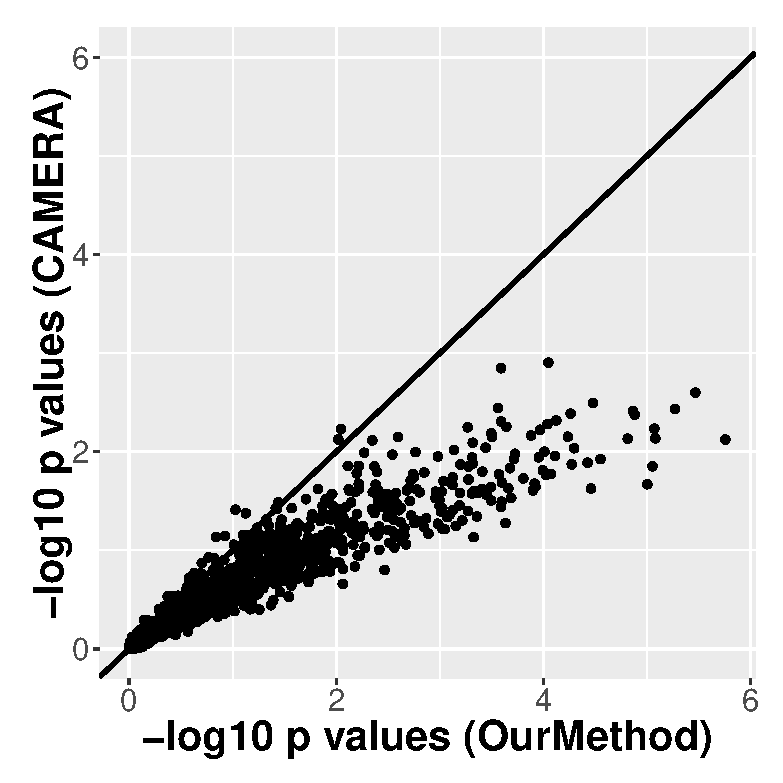
\includegraphics[width=5.5cm,height=5cm]{Figures/log10P_Camera.eps}
		 		 			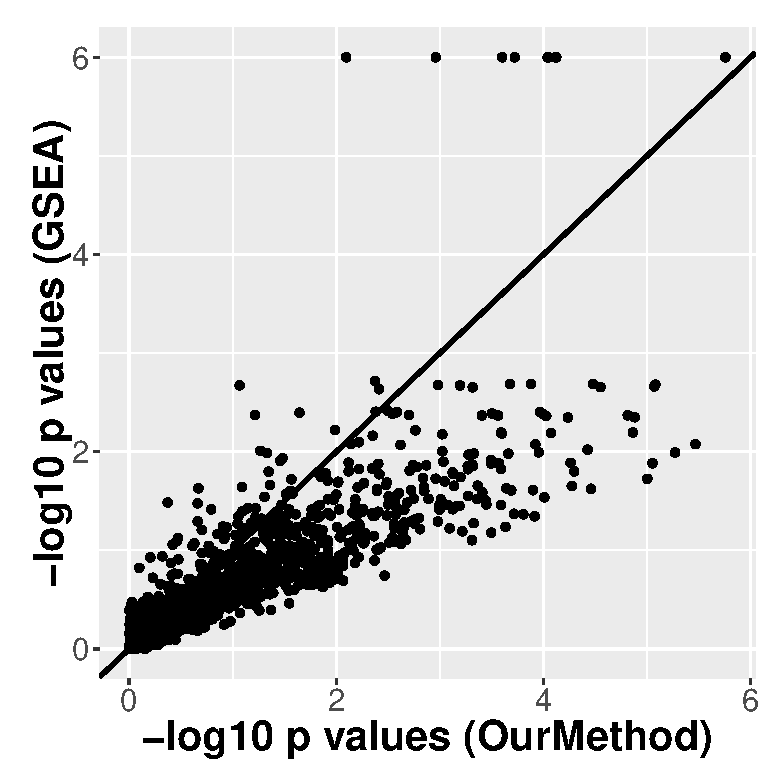
\includegraphics[width=5.5cm,height=5cm]{Figures/log10P_GSEA.eps}
		 		 			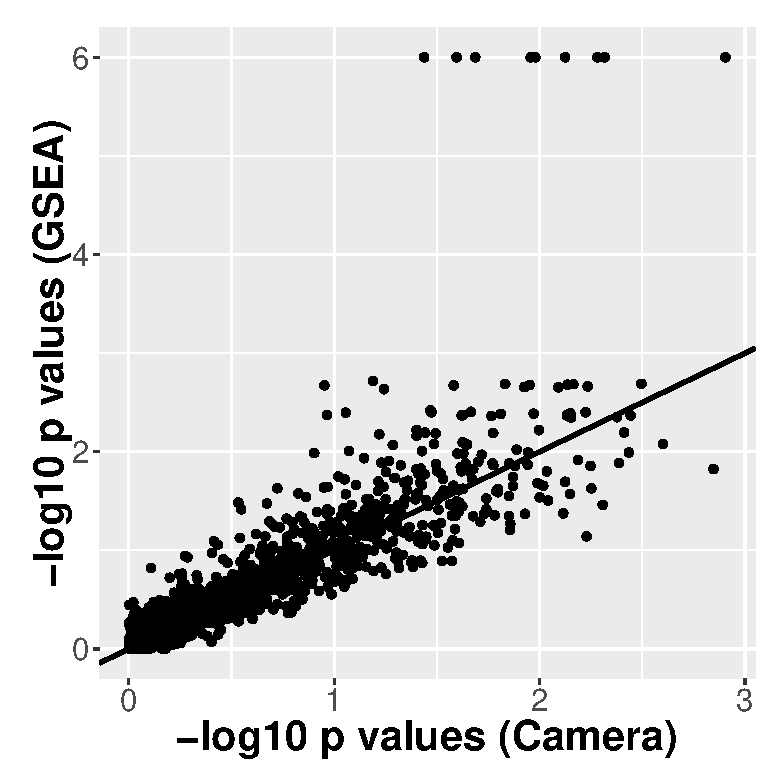
\includegraphics[width=5.5cm,height=5cm]{Figures/log10P_GSEA_CAMERA.eps}
		 		 		\end{center} 
		 		 	\end{figure} 
		 		 	
		  We report the top 30 enriched gene sets in Table \ref{table:top30}. Five enriched gene sets identified by GSEA are also present (noted by "$\ast$" in the table). Originally, \cite{labadorf2015rna} used the same HD data set to conduct enrichment analysis using topGo \citep{alexa2010topgo}. They found that the enriched gene sets they identified show a clear immune response and inflammation-related pattern, including REACTOME INNATE IMMUNE SYSTEM, PID IL4 2PATHWAY, and PID NFKAPPAB CANONICAL PATHWAY. These three gene sets rank 6,10 and 2 respectively in Table \ref{table:top30}.
		  
		   Many of our enriched gene sets have been shown to be closely related to HD pathogenesis. For example, the top enriched gene set by OurMethod, "PID SMAD2 3NUCLEAR PATHWAY" (see Table \ref{table:top30}), is responsible for regulation of nuclear SMAD2/3 signaling. \cite{katsuno2010disrupted} showed that nuclear SMAD2/3 are related to polyglutamine disease, which includes HD. The second enriched gene set, "PID NFKAPPAB CANONICAL PATHWAY", is a canonical NF-kappaB pathway, and its dysregulation causes HD immune dysfunction \citep{trager2014htt}. Also, \cite{marcora2010huntington} found that reduced transport of NF-kappaB out of dendritic spines and its activity in neuronal nuclei may contribute to the etiology of HD. 
		   %HD mutation can reduce the transport of NF-kappaB out of dendritic spines and its activity in neuronal nuclei and this reduction may contribute to the etiology of HD. 
		    Another gene set, "REACTOME INNATE IMMUNE SYSTEM", contributes to HD pathogenesis \citep{trager2014htt, labadorf2015rna}. \cite{diamanti2013whole} showed that "REACTOME TRANSCRIPTIONAL ACTIVITY OF SMAD2 SMAD3 SMAD4 HETEROTRIMER", a gene set involved in transcriptional activity of SMAD2/SMAD3:SMAD4 heterotrimer, is also enriched in their microarray study of HD pathology from blood samples of R6/2 at manifest stage and wild type littermate mice. For AKT signaling pathway, "BIOCARTA AKT PATHWAY", \cite{humbert2002igf} demonstrated that huntingtin is a substrate of AKT and that phosphorylation of huntingtin by AKT is crucial to mediate the neuroprotective effects of IGF-1. They also showed that AKT is altered in Huntington’s disease patients.  
			\cite{chiang2010modulation} demonstrated that the systematic downregulation of PPAR$\gamma$, related to "BIOCARTA PPARA PATHWAY", seems to play a critical role in the dysregulation of energy homeostasis observed in HD, and that PPAR$\gamma$ is a potential therapeutic target for this disease. For "REACTOME SIGNALING BY TGF BETA RECEPTOR COMPLEX",  \cite{kandasamy2011transforming} demonstrated that TGF-beta1 signaling appears to be a crucial modulator of neurogenesis in HD pathology and it can be a promising target for endogenous cell-based regenerative therapy. 
		   For "PID P53 DOWNSTREAM PATHWAY", \cite{ghose2011regulation} showed the likely involvement of NFkB (RelA), p53 and miRNAs in the regulation of cell death in HD pathogenesis. 
		 	 	
	
	
		{\scriptsize \begin{longtable}{p{3in}rp{0.5in}p{0.5in}rp{0.5in}p{0.5in}rp{0.5in}p{0.5in}lp{0.1in}}
				\label{table:top30} \\
				\caption{Top Enriched gene sets} \\
				\hline
				\hline
				Gene Set & Size & $\rho_1$ & $\rho_2$ & $\rho_3$ & $p$-value & FDR & \\ 
				\hline
		PID SMAD2 3NUCLEAR PATHWAY & 79 & 0.071 & 0.011 & 0.017 & 7.5E-07 & 9.9E-04 & $\ast$ \\ 
		PID NFKAPPAB CANONICAL PATHWAY & 22 & 0.124 & 0.011 & 0.020 & 2.4E-06 & 1.6E-03 &  \\ 
		REACTOME YAP1 AND WWTR1 TAZ STIMULATED GENE EXPRESSION & 23 & 0.130 & 0.011 & 0.018 & 4.4E-06 & 1.7E-03 &  \\ 
		REACTOME SIGNALING BY TGF BETA RECEPTOR COMPLEX & 60 & 0.045 & 0.011 & 0.015 & 7.3E-06 & 1.7E-03 &  \\ 
		BIOCARTA NTHI PATHWAY & 23 & 0.124 & 0.011 & 0.024 & 7.5E-06 & 1.7E-03 &  \\ 
		REACTOME INNATE IMMUNE SYSTEM & 209 & 0.048 & 0.011 & 0.010 & 7.8E-06 & 1.7E-03 &  \\ 
		KEGG PATHWAYS IN CANCER & 311 & 0.029 & 0.011 & 0.010 & 8.9E-06 & 1.7E-03 &  \\ 
		REACTOME DOWNSTREAM TCR SIGNALING & 31 & 0.095 & 0.011 & 0.013 & 1.2E-05 & 1.9E-03 &  \\ 
		KEGG NOD LIKE RECEPTOR SIGNALING PATHWAY & 55 & 0.054 & 0.011 & 0.010 & 1.3E-05 & 1.9E-03 &  \\ 
		PID IL4 2PATHWAY & 59 & 0.086 & 0.011 & 0.012 & 1.4E-05 & 1.9E-03 &  \\ 
		KEGG TGF BETA SIGNALING PATHWAY & 82 & 0.062 & 0.011 & 0.013 & 2.7E-05 & 3.3E-03 &  \\ 
		BIOCARTA 41BB PATHWAY & 14 & 0.095 & 0.011 & 0.023 & 3.2E-05 & 3.4E-03 &  \\ 
		PID P53 DOWNSTREAM PATHWAY & 131 & 0.052 & 0.011 & 0.013 & 3.4E-05 & 3.4E-03 &  \\ 
		REACTOME TCR SIGNALING & 48 & 0.098 & 0.011 & 0.016 & 3.6E-05 & 3.5E-03 &  \\ 
		REACTOME ACTIVATED TLR4 SIGNALLING & 87 & 0.027 & 0.011 & 0.010 & 4.9E-05 & 4.2E-03 &  \\ 
		REACTOME TOLL RECEPTOR CASCADES & 110 & 0.038 & 0.011 & 0.010 & 5.2E-05 & 4.2E-03 &  \\ 
		REACTOME TRANSCRIPTIONAL REGULATION OF WHITE ADIPOCYTE DIFFERENTIATION & 69 & 0.015 & 0.011 & 0.010 & 5.4E-05 & 4.2E-03 &  \\ 
		BIOCARTA TID PATHWAY & 18 & 0.125 & 0.011 & 0.017 & 5.7E-05 & 4.2E-03 &  \\ 
		BIOCARTA ALK PATHWAY & 34 & 0.064 & 0.011 & 0.011 & 7.4E-05 & 5.1E-03 & $\ast$ \\ 
		REACTOME SMAD2 SMAD3 SMAD4 HETEROTRIMER REGULATES TRANSCRIPTION & 25 & 0.102 & 0.011 & 0.021 & 7.6E-05 & 5.1E-03 & $\ast$ \\ 
		REACTOME TRANSCRIPTIONAL ACTIVITY OF SMAD2 SMAD3 SMAD4 HETEROTRIMER & 36 & 0.079 & 0.011 & 0.021 & 8.3E-05 & 5.1E-03 &  \\ 
		BIOCARTA AKT PATHWAY & 20 & 0.023 & 0.011 & 0.010 & 8.8E-05 & 5.1E-03 & $\ast$ \\ 
		ST TUMOR NECROSIS FACTOR PATHWAY & 28 & 0.039 & 0.011 & 0.016 & 9.0E-05 & 5.1E-03 & $\ast$ \\ 
		PID ANGIOPOIETIN RECEPTOR PATHWAY & 50 & 0.082 & 0.011 & 0.013 & 9.3E-05 & 5.1E-03 &  \\ 
		KEGG P53 SIGNALING PATHWAY & 65 & 0.037 & 0.011 & 0.007 & 9.7E-05 & 5.1E-03 &  \\ 
		KEGG APOPTOSIS & 82 & 0.041 & 0.011 & 0.009 & 1.0E-04 & 5.1E-03 &  \\ 
		BIOCARTA PPARA PATHWAY & 53 & 0.026 & 0.011 & 0.008 & 1.1E-04 & 5.2E-03 &  \\ 
		REACTOME MYD88 MAL CASCADE INITIATED ON PLASMA MEMBRANE & 78 & 0.026 & 0.011 & 0.010 & 1.1E-04 & 5.2E-03 &  \\ 
		PID BCR 5PATHWAY & 64 & 0.064 & 0.011 & 0.016 & 1.2E-04 & 5.3E-03 &  \\ 
		PID HIF1 TFPATHWAY & 64 & 0.067 & 0.011 & 0.011 & 1.2E-04 & 5.3E-03 &  \\ 
		
		\hline	
				\hline
		\multicolumn{7}{l}{$\rho_1$: average sample correlation between genes in the test set. }	 \\	
		\multicolumn{7}{l}{$\rho_2$: average sample correlation between genes in the background set. }	 \\	
		\multicolumn{7}{l}{$\rho_3$: average sample correlation between two genes, one from the test set and the other from the background set. }	 \\	
		\multicolumn{7}{l}{ ~~$\ast$: enriched gene sets identified by GSEA.}	 \\	
				\end{longtable}
		}
		

		 	



		\subsubsection*{Male vs Female Lymphoblastoid Cells Data}
		We analyzed the mRNA expression profiles data from lymphoblastoid cell lines derived from 17 females and 15 males. \cite{subramanian2005gene} examined this data set with their GSEA method, testing the enrichment of the  cytogenetic gene sets (C1). C1 includes 24 sets, one for each of the 24 human chromosomes, and 295 sets corresponding to cytogenetic bands. \cite{subramanian2005gene} expected to find gene sets in chromosome Y to be correlated with the comparison "\text{male}$>$\text{female}". We run enrichment analysis with three tests (OurMethod, GSEA and CAMERA). In Table \ref{table:gender}, we summarized all the gene sets called significant by at least one test for the nominal $p$-value of 0.01. Three gene sets, one from chromosome Y and two Y bands, are found to be enriched by all three tests for the "\text{male}$>$\text{female}" comparison. Interestingly, OurMethod identified another Y band, chrYp22, as enriched. In fact, the four gene sets in Table \ref{table:gender} identified as significant by OurMethod are the only four containing at least 3 genes in C1 and corresponding to chromosome Y and Y bands. However, GSEA produced small nominal $p$-values for gene sets ( How to explain this? can we rule out those genes for not being related to Y or Y band?).
		
		\begin{table}[ht]
		%	\label{table:gender} 
			\centering
			\caption{Gene sets for lymphoblastoid cells data.}
		\begin{tabular}{lrrr c rr c rr} \hline\hline 
		 & &  \multicolumn{2}{c}{OurMethod} & & \multicolumn{2}{c}{GSEA}	& & \multicolumn{2}{c}{CAMERA} \\	
		 \cline{3-4}  \cline{6-7} \cline{9-10}
		Gene set & Size & $p$-value & FDR & & $p$-value & FDR & &$p$-value & FDR \\ 
		\hline
		chrY & 40 & $<0.001$ & $<0.001$ & &$<0.001$ & $<0.001$ & & $<0.001$ & 0.002 \\ 
		chrYq11 & 16 & $<0.001$ & $<0.001$& & $<0.001$ & $<0.001$ & & $<0.001$ & $<0.001$ \\ 
		chrYp11 & 18 & $<0.001$ & $<0.001$ & & $<0.001$ & $<0.001$& & $<0.001$ & 0.028 \\ 
		chrYp22 & 8 & $<0.001$ & 0.036& & 0.012 & 0.503 & & 0.010 & 0.762 \\ 
		chr7p11 & 8 & 0.049 & 0.835 & & 0.006 & 0.352 & & 0.101 & 0.998 \\ 
		chr11p12 & 5 & 0.065 & 0.835& & 0.008 & 0.388 & & 0.115 & 0.998 \\ 
		chrXp22 & 76 & 0.072 & 0.835& & 0.004 & 0.295 & & 0.581 & 0.998 \\  
		\hline\hline
			\end{tabular}
			\label{table:gender}
		\end{table}
		
	\section{Discussion}
		 
		 There are many methods developed for gene set tests (see reviews by \cite{huang2009bioinformatics, khatri2012ten, tarca2013comparison}). Using the terminology of \cite{khatri2012ten}, these methods generally fall into three categories: \textit{over-representation analysis}, \textit{functional class scoring} and \textit{pathway topology}. The over-representation analysis evaluates a fraction of genes among a set of pre-selected interesting genes (e.g., differentially expressed genes between treatment versus control samples). The test is usually conducted in the form of $2\times 2$ table, for example, GOstat of \cite{klebanov2007multivariate} and GO:TermFinder of \cite{tian2005discovering}. However, the over-representation analysis methods have inherent limitations such as information loss by choosing arbitrary threshold (e.g., $p$-value $< 0.05$), or problematic assumption of independence of genes (\cite{goeman2007analyzing, wu2012camera}). The functional class scoring performs three-stage analysis \citep{khatri2012ten}: on the first stage, a \textit{gene-level statistic} that measures the association between the expression profiles and the experimental design variables is calculated for each gene; such gene-level statistics include, among others, signal-to-noise ration \citep{subramanian2005gene}, moderated $t$ statistics \citep{Smyth2004moderated} and  $Z$-score \citep{efron2007correlation}. On the second stage, a \textit{set-level statistic} is calculated by using gene-level statistics and prior information about the test set (i.e., whether the gene belongs to the set) as input. On the last stage, a $p$-value is assigned to the test set by comparing the set-level statistic to its reference distribution.  (Rewrite this part)		 
		 The pathway topology will not be discussed in this paper (\cite{khatri2012ten, tarca2013comparison})
		 	
	\section{Conclusion}\label{section:conclusion}
	
	\section{AcknowledgeMents}\label{section:acknowledgement}
	
	\section{Appendix}\label{section:appendix}
	
	First $E(\Delta_i) = E(Z_i\delta_i) = E(Z_i)E(\delta_i) = p_i\mu_{\delta}$. Next note that  
	\[\text{Var}(\Delta_i) = E[(Z_i\delta_i)^2]- [E(Z_i\delta_i)]^2 = \text{Var}(Z_i)[E(\delta_i)]^2 + \left[(EZ_i)^2 + \text{Var}(Z_i)\right]\text{Var}(\delta_i) =p_i\sigma_{\delta}^2 + p_i(1-p_i)\mu_{\delta}^2\]
	
	Let $T_i=\bar{Y}_{i,2}-\bar{Y}_{i,1}$ be the difference in mean expression levels between the treatment group and the control group. We have 
	\[E(T_i) = E(\bar{Y}_{i,2})-E(\bar{Y}_{i,1}) = E(\Delta_i) = E(Z_i\delta_i) = p_i\mu_{\delta}\]
	The covariance between two genes $i_1$ and $i_2$ is given by (I HAVE CONCERNS HERE, IS IT VALID TO ASSUME THAT DE EFFECTS ARE INDEPENDENT BETWEEN GENES?  WE SEE CO-EXPRESSION!! OR WE'VE ALREADY TAKEN THAT INTO ACCOUNT BY CORRELATION BETWEEN GENES"), 
	
				\begin{equation}
					\begin{aligned}
						\text{Cov}(T_{i_1}, T_{i_2}) & = E\left[\text{Cov}(T_{i_1}, T_{i_2}|\Delta_{i_1}, \Delta_{i_2}) \right]  + \text{Cov}\left[E(T_{i_1}|\Delta_{i_1}), E(T_{i_2}|\Delta_{i_2})\right] \\
						& = E\left(\frac{1}{n_1}\rho_{i_1,i_2} + \frac{1}{n_2}\rho_{i_1,i_2}\right) + \text{Cov}(\Delta_{i_1}, \Delta_{i_2})\\
						& = \left(\frac{1}{n_1} + \frac{1}{n_2}\right)\rho_{i_1,i_2}
					\end{aligned}
				\end{equation}
				For gene $i$, the variance $\text{Var}(T_i) = \text{Var}(\bar{Y}_{i, 1}) + \text{Var}(\bar{Y}_{i, 2})$, with
				\[\text{Var}(\bar{Y}_{i, 1}) = \frac{1}{n_1}\] 
				\begin{equation}
					\begin{aligned}
						\text{Var}(\bar{Y}_{i, 2}) & = \frac{1}{n_2^2}\left[\sum_{j=1}^{n_2}\text{Var}(Y_{ij2}) + 2\sum_{1\leq j_1<j_2 \leq n_2} \text{Cov}(Y_{ij_12}, Y_{ij_22})\right] \\
						& = \frac{1}{n_2}\text{Var}(Y_{ij2}) + \frac{n_2-1}{n_2} \text{Cov}(Y_{ij_12}, Y_{ij_22})\\
						& = \frac{1}{n_2}\left[E\left(\text{Var}(Y_{ij2}|\Delta_i)\right) + \text{Var}\left(E(Y_{ij2}|\Delta_i)\right)\right] \\ \text{~~~} &+\frac{n_2-1}{n_2}\left[E\left(\text{Cov}(Y_{ij_12}, Y_{ij_22}|\Delta_i)\right) + \text{Cov}\left(E(Y_{ij_12}|\Delta_i), E(Y_{ij_22}|\Delta_i)\right)\right] \\
						& = \frac{1}{n_2} + \text{Var}(\Delta_i)
					\end{aligned}
				\end{equation}
				Therefore $\text{Var}(T_i)  = \frac{1}{n_1} + \frac{1}{n_2} + \text{Var}(\Delta_i)$, and it follows that
				\begin{equation}\label{eq:tvar}
					\text{Cov}(\bm T) =  \bm D + \sigma_2^2\bm C 
				\end{equation}
				where $\bm D$ is a diagonal matrix with $\text{Var}(\Delta_i) =p_i\sigma_{\delta}^2 + p_i(1-p_i)\mu_{\delta}^2$ as its $i$th diagonal element, and $\sigma_2^2 = \left(\frac{1}{n_1} + \frac{1}{n_2}\right)$.

				
				
				
								

\newpage
\bibliographystyle{apalike}
\bibliography{mybib}
	
\end{document}



	our main point
	\begin{enumerate}
		\item section 1:  introduction begins here (suggestions: try writing your introductions last).
		\begin{enumerate}
			\item what is my topic (question)?
			\item why is it important?
			\item how will I plan to proceed with my
		\end{enumerate}
		\item previous comparative gene set enrichment analysis does not take....
		\item we propose a method that allows DE within the test set as well as the background gene set.
	\end{enumerate}
	
